%!TEX root = draft.tex
\section{Scaling} \label{sec:scaling}
In this section we present some results that demonstrate the scalability of our algorithms. All of our tests were ran on the Stampede cluster at Texas Advanced Computing Center (TACC) where we are limited to $4096$ cores at most. Each node of Stampede has 2 eight-core Xenon E5-2680 processors clocked at 2.7 GHz with 32 GB of DDR3-1600 MHz memory and interconnected using an InfiniBand network card. Unless mentioned otherwise, in all the tests we have used all 16 cores of every node. Finally, in all cases we report the maximum wall time recorded using PETSc's logging interface which has a temporal resolution of roughly $0.1 \: \mu s$.

\subsection{Interpolation}
In this section we show the results for a simple test to measure the scalability of the interpolation algorithm \ref{alg:interpolation}. The test consists in interpolating a function at a number of random points on a randomly refined Octree in three spatial dimensions. We consider two cases, a small test on a level 9 tree with roughly 20M cells and 33M nodes and larger test on a level 13 tree with roughly 128M cells and 280M nodes. In both cases the number of randomly generated points is chosen to be equal to the number of nodes and the stablized second-order interpolation of \cite{Min;Gibou:07:A-second-order-accur} is performed 10 times to smooth out possible timing fluctuations.

To simulate the effect of different CFL numbers, we generate the random points such that on each processor $\alpha\%$ of them are located outside the processor boundary and will thus initiate communication. Scaling results are presented for $\alpha = 5 \%$ and $\alpha = 95\%$ for both the small and large problems in figure \ref{fig:interpolation}. Excellent scaling is obtained for the small problem for $P = 16-512$ even when $95\%$ of the interpolation points belong to a remote processor. For the larger problem, the communication overhead prevents the algorithm from scaling beyond $4096$ processors when $\alpha = 95\%$. Note that for $\alpha = 5\%$, even though some sections of the algorithm stop scaling, the overall algorithm still scales since the local work dominates the timing. This illustrates the effectiveness of the non-blocking communication pattern of algorithm \ref{alg:interpolation}.

\begin{figure}[htbp]
	\begin{center}
		\subfigure[$N_G = 33$M, $\alpha = 5\%$]{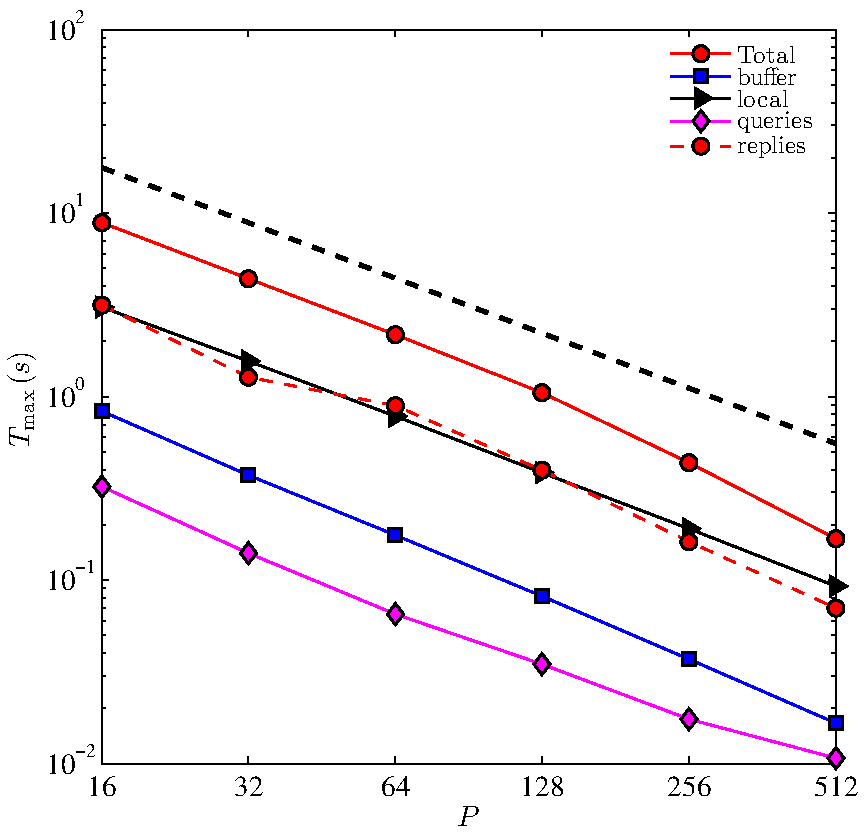
\includegraphics[width = 0.45 \textwidth] {figures/interpolation_small_05.pdf}}
		\subfigure[$N_G = 33$M, $\alpha = 95\%$]{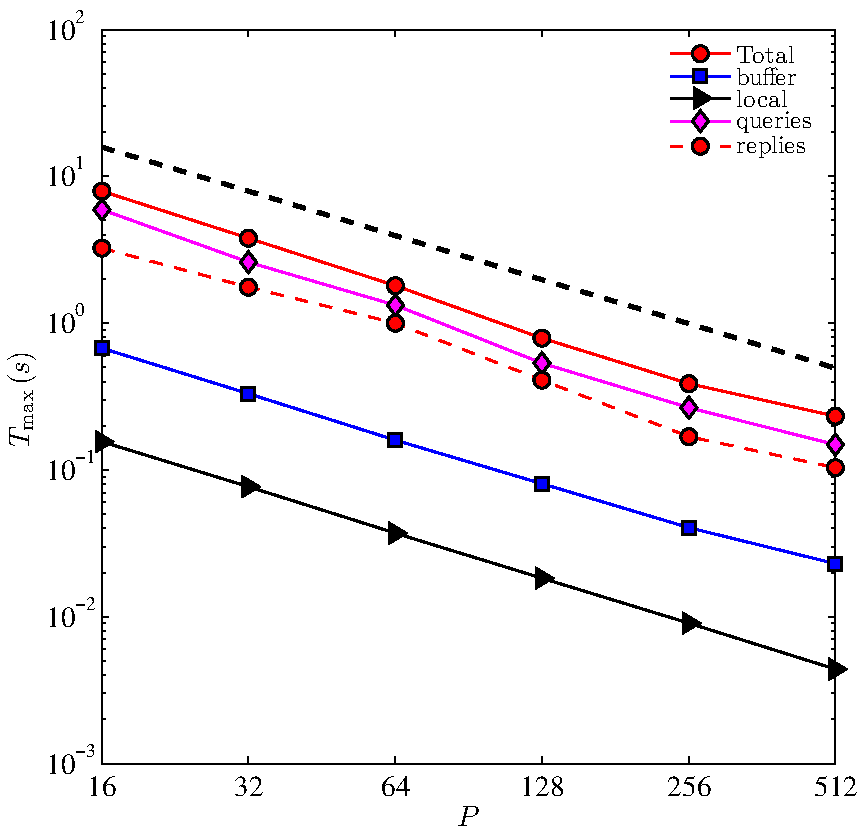
\includegraphics[width = 0.45 \textwidth] {figures/interpolation_small_95.pdf}}
		\\
		\subfigure[$N_G = 280$M, $\alpha = 5\%$]{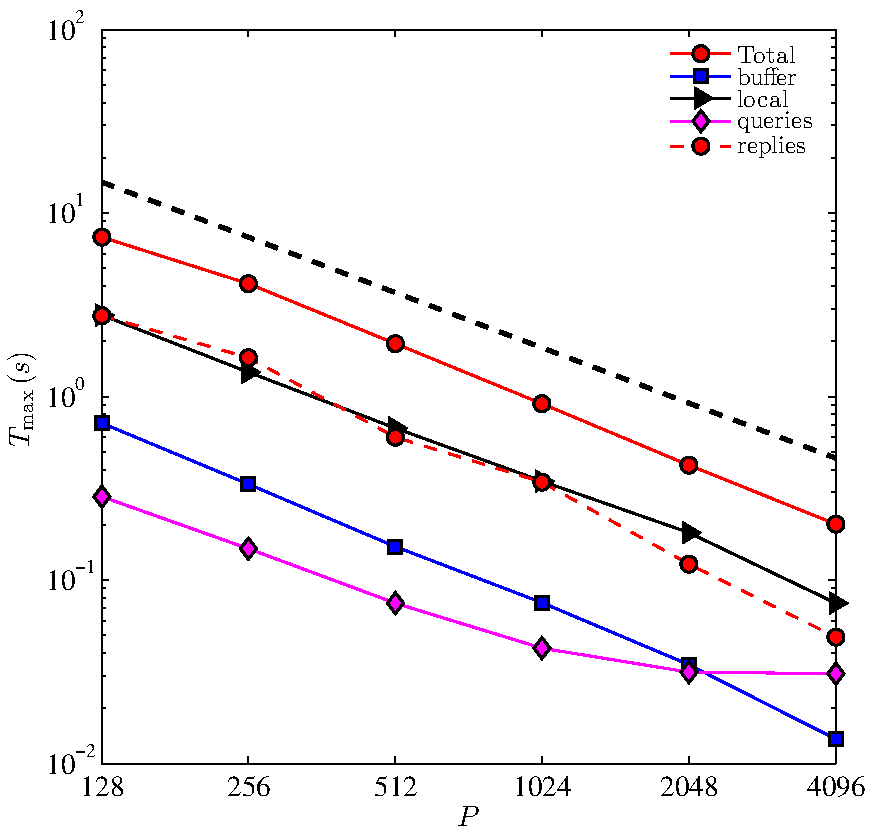
\includegraphics[width = 0.45 \textwidth] {figures/interpolation_large_05.pdf}}
		\subfigure[$N_G = 280$M, $\alpha = 95\%$]{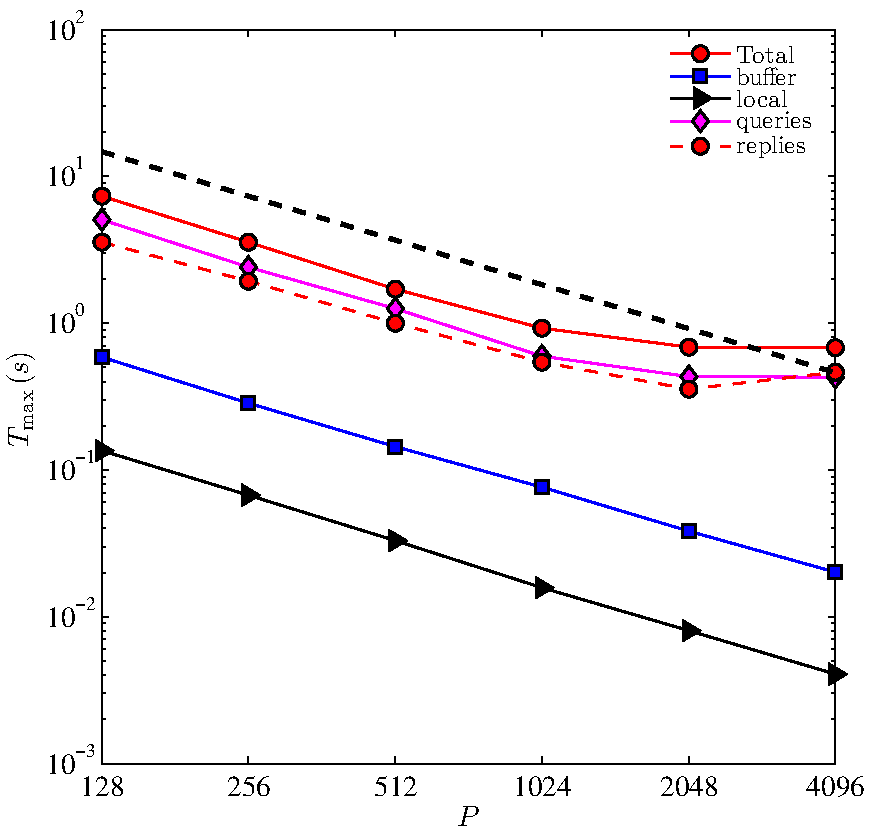
\includegraphics[width = 0.45 \textwidth] {figures/interpolation_large_95.pdf}}
	\end{center}
	\caption{Strong scaling of algorithm \ref{alg:interpolation} for several tests where $N_G$ denotes the number of random interpolation points (which is the same as the number of nodes in the Octree) and $\alpha$ denotes the percentage of these points that are remote for each processor. Here ``Total'' represents the total time spent in the interpolation while ``buffer'', ``local'', ``queries'', and ``replies'' represent the the timing for different sections (c.f. algorithm \ref{alg:interpolation}). The results indicate excellent scaling for the small test (a-b) and for the large test when $\alpha = 5\%$ (c). For the extreme case (d) the algorithm stops scaling at $4096$ processors due to communication overhead.}
	\label{fig:interpolation}
\end{figure}

\subsection{Semi-Lagrangian}
To test the scalability of the Semi-Lagrangian algorithm \ref{alg:semi-lagrangian} we consider a slightly modified version of the Enright's rotation test \cite{Enright;Fedkiw;Ferziger;etal:02:A-Hybrid-Particle-Le}, i.e. we advect a sphere of radius 0.35 located at $(0.4, 0.4, 0.4)$ with a divergence free velocity field given by:
\bean
u(x,y,z) &=& 2\sin(\pi x)^2 \sin(2\pi y) \sin(2 \pi z), \\
v(x,y,z) &=& -\sin(\pi y)^2 \sin(2\pi x) \sin(2 \pi z),\\
w(x,y,z) &=& -\sin(\pi z)^2 \sin(2\pi x) \sin(2 \pi y). 
\eean
To understand the effect of the CFL number on the scalability of the algorithm we perform one step of the Semi-Lagrangian algorithm for $\text{CFL} = 1$, $\text{CFL} = 10$, and $\text{CFL} = 100$. We also perform the test for two different initial girds, a small grid with maximum level $l_\text{max} = 10$ and a large grid with maximum level $l_\text{max} = 12$. After one advection step, these grids have approximately 15M and 255M nodes, respectively. 
\begin{table}[htbp]
	\begin{minipage}{.5\linewidth}
		\begin{center}
		\begin{tabular}{|c|cccccc|}
			\hline
				CFL & 16 & 32 & 64 & 128 & 256 & 512 \\
				\hline
				1   & 2 & 2 & 3 & 3 & 3 & 3 \\
				10  & 3 & 3 & 3 & 3 & 3 & 3 \\
				100 & 6 & 6 & 6 & 6 & 6 & 6 \\
			\hline
		\end{tabular}
		\caption*{(a) $l_\text{max} = 10$}
		\end{center}
	\end{minipage}%
	\begin{minipage}{.5\linewidth}
		\begin{center}
		\begin{tabular}{|c|cccccc|}
			\hline
				CFL & 128 & 256 & 512 & 1024 & 2048 & 4096 \\
			\hline
				1   & 3 & 3 & 3 & 3 & 3 & 3 \\
				10  & 3 & 3 & 4 & 4 & 4 & 4 \\
				100 & 6 & 6 & 6 & 6 & 6 & 7 \\
			\hline
		\end{tabular}
		\caption*{(b) $l_\text{max} = 12$}
		\end{center}
	\end{minipage}	
	\caption{Number of iterations required for the grid construction in algorithm \ref{alg:semi-lagrangian} for the rotation test on a (a) level-10 and (b) level-12 Octree with approximately 15M and 255M nodes, respectively. Note how the iteration count increases with the CFL number but is almost independent of the number of processors. The slight dependence between the number of iterations and the number of processors is most likely due to the dependence of round-off errors on the number of processors. Nonetheless, close examination of the Octrees generated (data not shown) reveals that they are identical and independent of the number of processors used to perform the test.}
	\label{tab:semilagrangian}
\end{table}

Table \ref{tab:semilagrangian} illustrates the dependence of the number of iterations required to build the grid on the CFL number; as the CFL is increased, the interface travels a farther distance which necessitates more iterations to generate the grid. Note that the apparent dependence on the number of processors is most likely due to round-off errors during the interpolation and/or backtracking steps. Figures \ref{fig:semilagrangian_small} and \ref{fig:semilagrangian_large} illustrate the scalability of the algorithm for the small and large problems, respectively. To enable meaningful comparisons between different CFL numbers and number of processors, the maximum time has been scaled by the number of iterations required for the grid construction as reported in table \ref{tab:semilagrangian}. For both problems, excellent scalability is observed for $\text{CFL} = 1$ and $\text{CFL} = 10$. The algorithm even shows good scalability when taken to the extreme, i.e. for $\text{CFL} = 100$.

An increase in the CFL number has two effects on the algorithm. First, a larger fraction of the departure points lands in the domains of remote processors. Moreover, these points are potentially dispersed across a larger number of processors. This means that both the number of MPI messages and their volume increase as the CFL number increases. Second, as more points are shipped to remote processors for interpolation, there is a greater chance that the interpolation load is imbalanced across processors. This is especially true for regions of space in which the streamlines cluster. Both factors contribute to decrease the scalability of the algorithm at large CFL numbers. 
\begin{figure}[htbp]
	\begin{center}
		\subfigure[Semi-Lagrangian, $\text{CFL} = 1$]{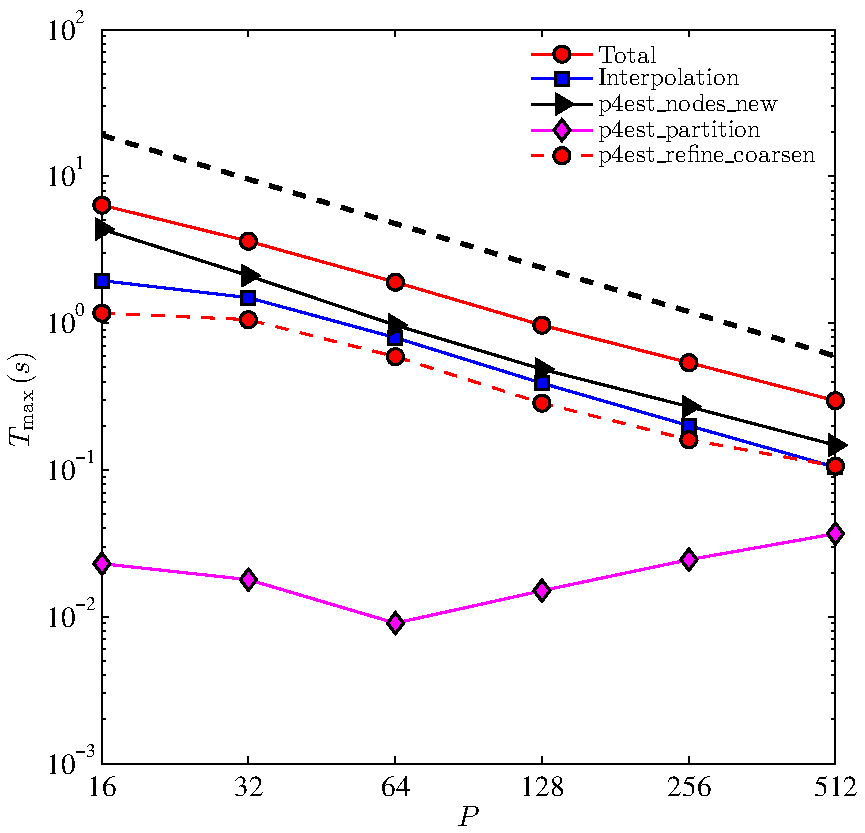
\includegraphics[width = 0.3 \textwidth] {figures/SL_Small_1_SemiLagrangian.pdf}}
		\subfigure[Semi-Lagrangian, $\text{CFL} = 10$]{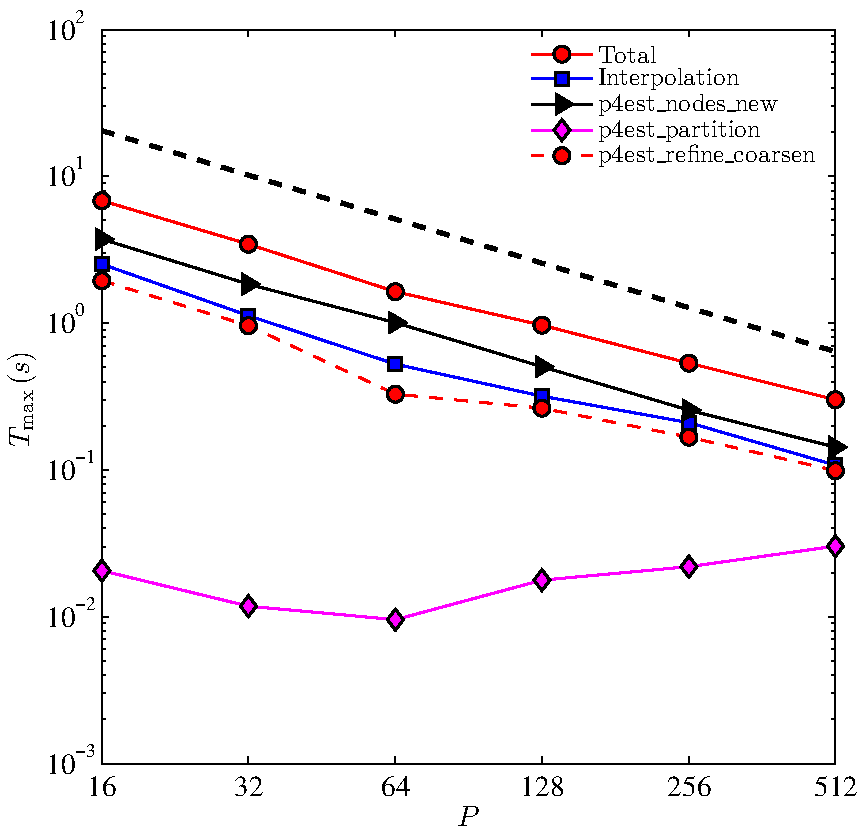
\includegraphics[width = 0.3 \textwidth] {figures/SL_Small_10_SemiLagrangian.pdf}}
		\subfigure[Semi-Lagrangian, $\text{CFL} = 100$]{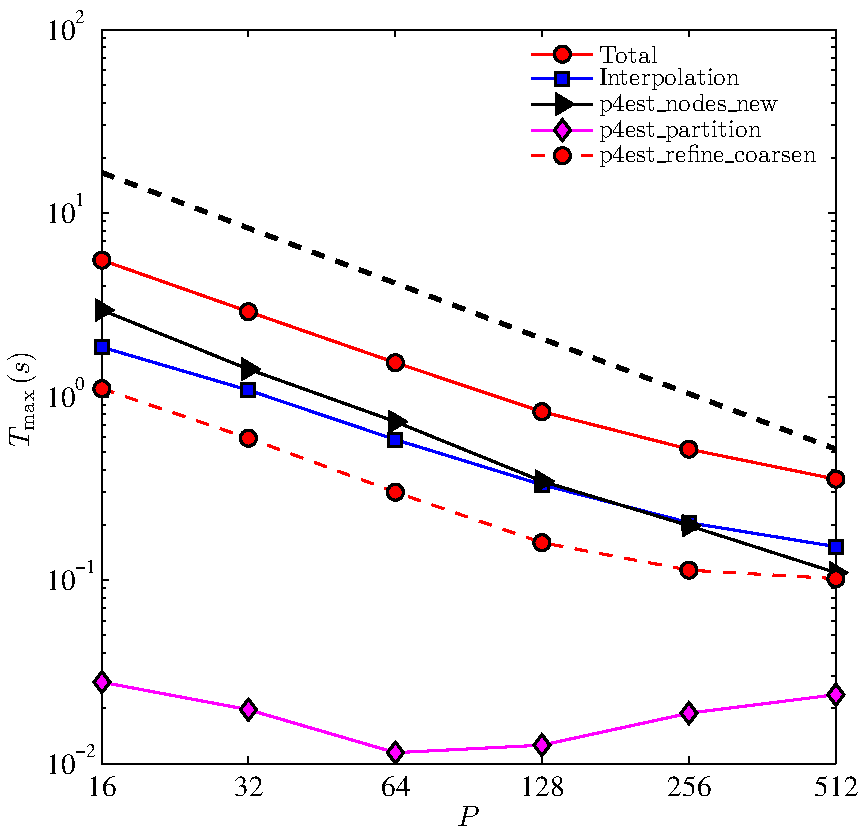
\includegraphics[width = 0.3 \textwidth] {figures/SL_Small_100_SemiLagrangian.pdf}}
		\\
		\subfigure[Interpolation, $\text{CFL} = 1$]{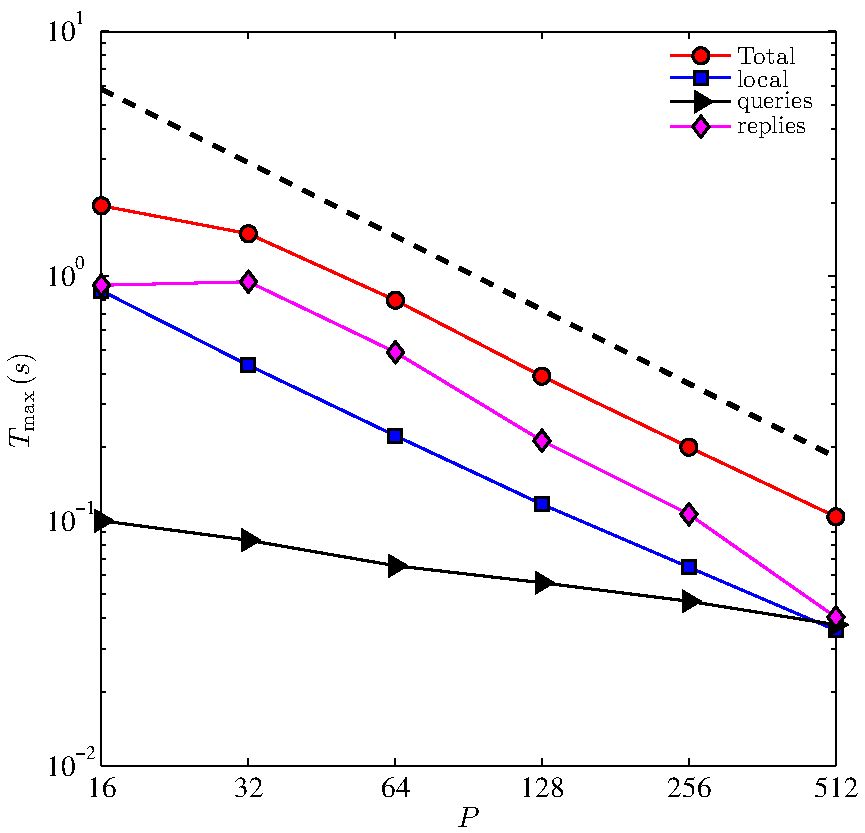
\includegraphics[width = 0.3 \textwidth] {figures/SL_Small_1_Interpolation.pdf}}
		\subfigure[Interpolation, $\text{CFL} = 10$]{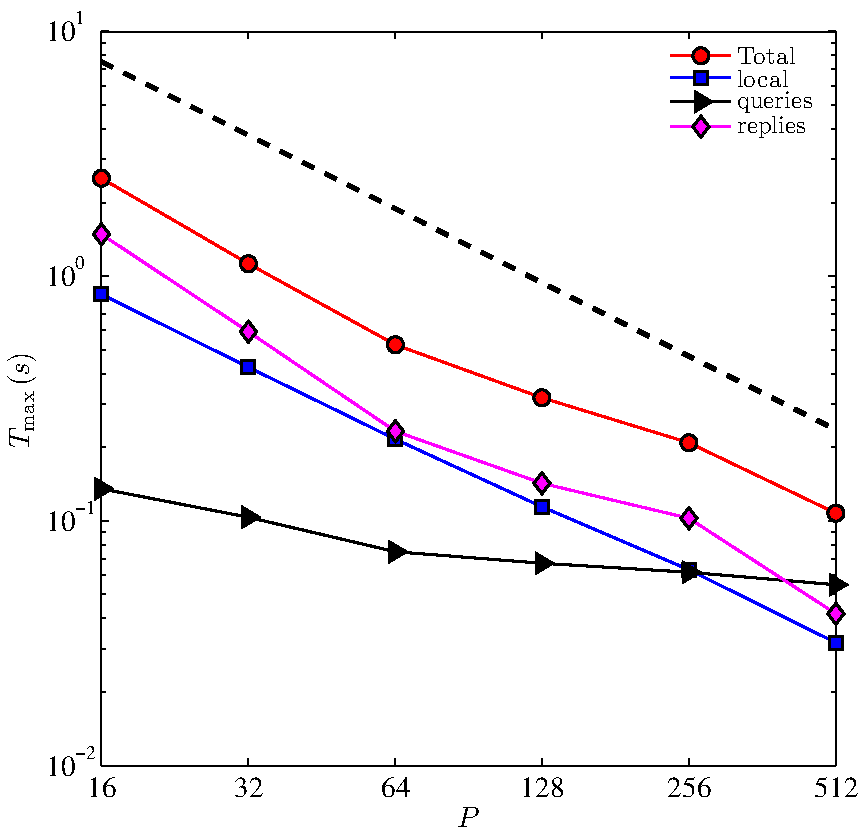
\includegraphics[width = 0.3 \textwidth] {figures/SL_Small_10_Interpolation.pdf}}
		\subfigure[Interpolation, $\text{CFL} = 100$]{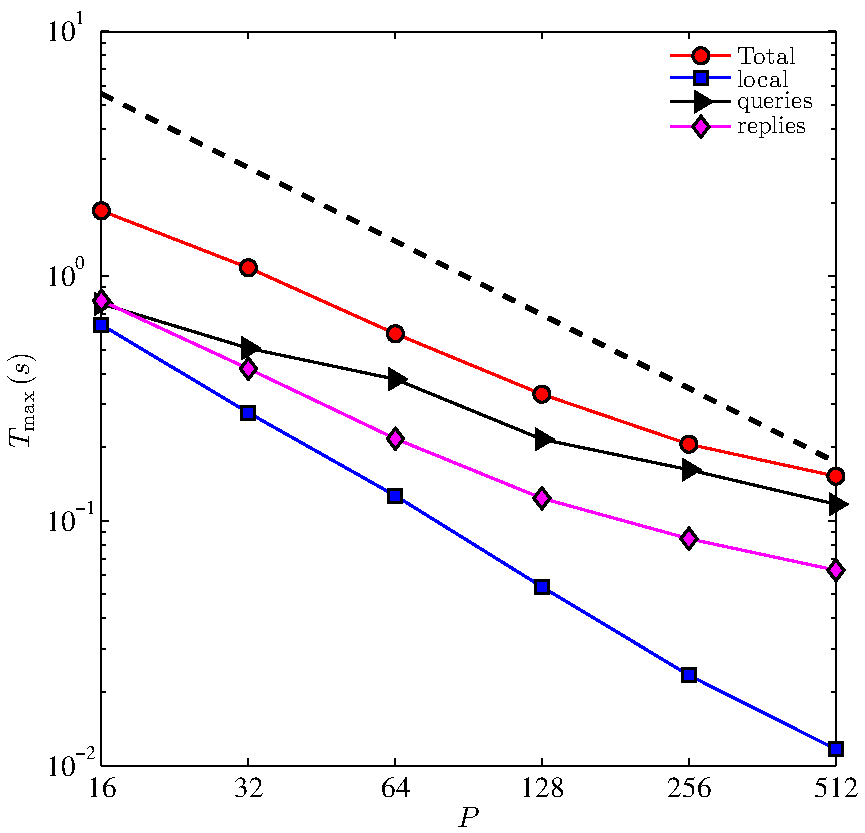
\includegraphics[width = 0.3 \textwidth] {figures/SL_Small_100_Interpolation.pdf}}
	\end{center}
	\caption{Strong scaling of a single iteration of algorithm \ref{alg:semi-lagrangian} for the rotation test on a level-10 Octree with approximately 13M cells and 15M nodes. Top row: scaling of the various components of the algorithm for (a) $\text{CFL} = 1$, (b) $\text{CFL} = 10$, and (c) $\text{CFL} = 100$. Bottom row: breakdown of the various components of the interpolation phase for the same CFL numbers. Note that the maximum time has been scaled by the number of iterations required to build the tree (c.f. table \ref{tab:semilagrangian}).}
	\label{fig:semilagrangian_small}
\end{figure}

\begin{figure}[htbp]
	\begin{center}
		\subfigure[Semi-Lagrangian, $\text{CFL} = 1$]{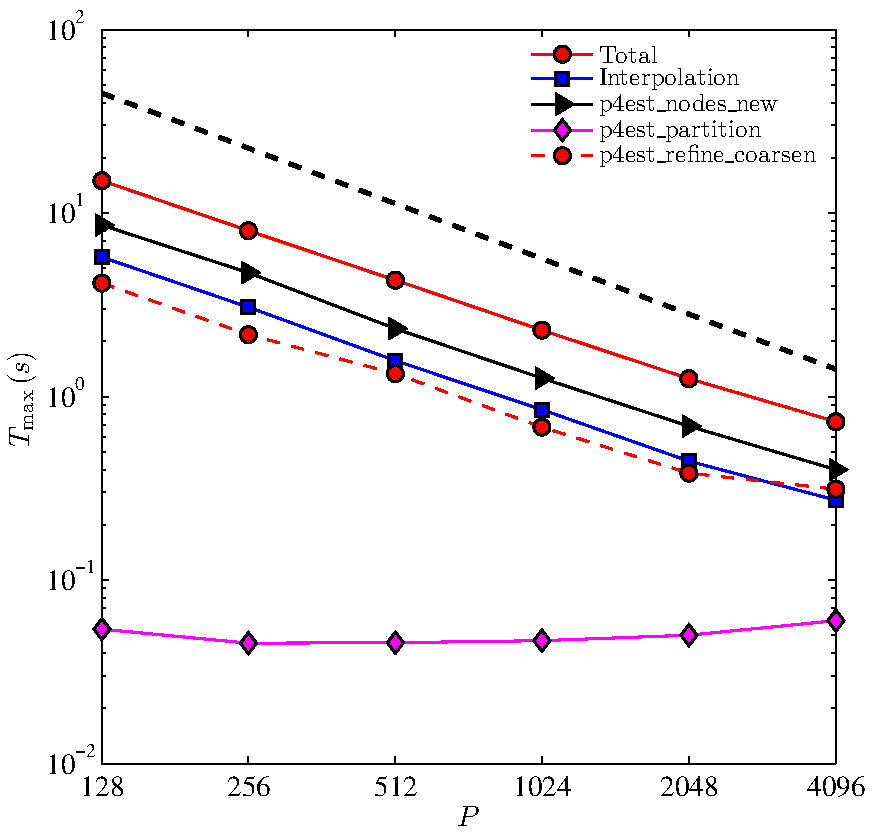
\includegraphics[width = 0.3 \textwidth] {figures/SL_Large_1_SemiLagrangian.pdf}}
		\subfigure[Semi-Lagrangian, $\text{CFL} = 10$]{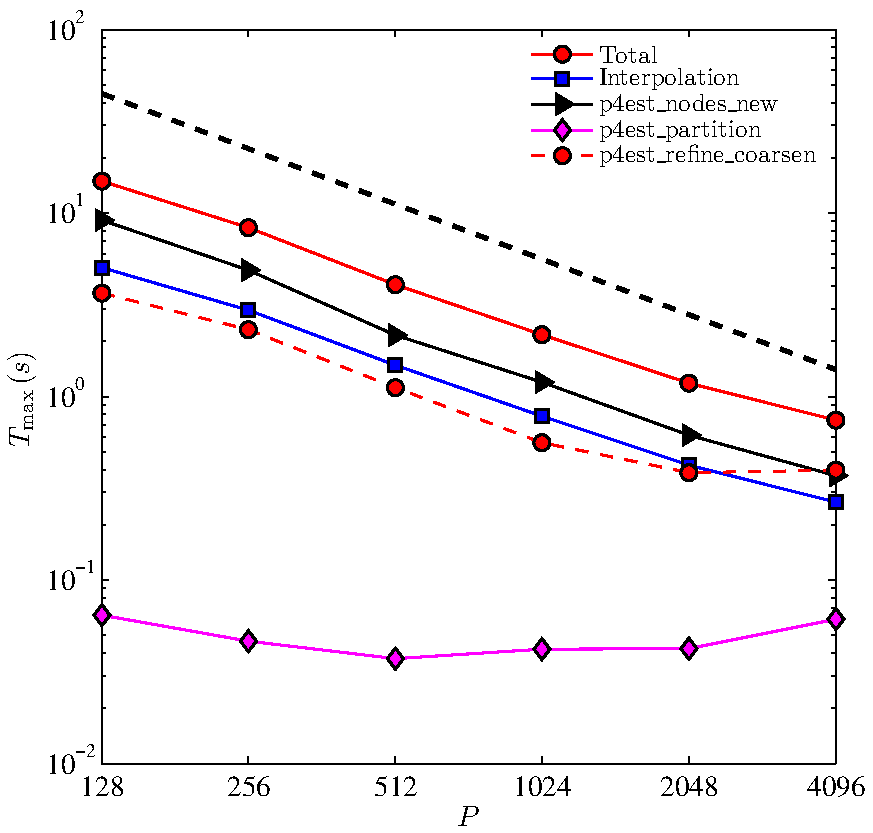
\includegraphics[width = 0.3 \textwidth] {figures/SL_Large_10_SemiLagrangian.pdf}}
		\subfigure[Semi-Lagrangian, $\text{CFL} = 100$]{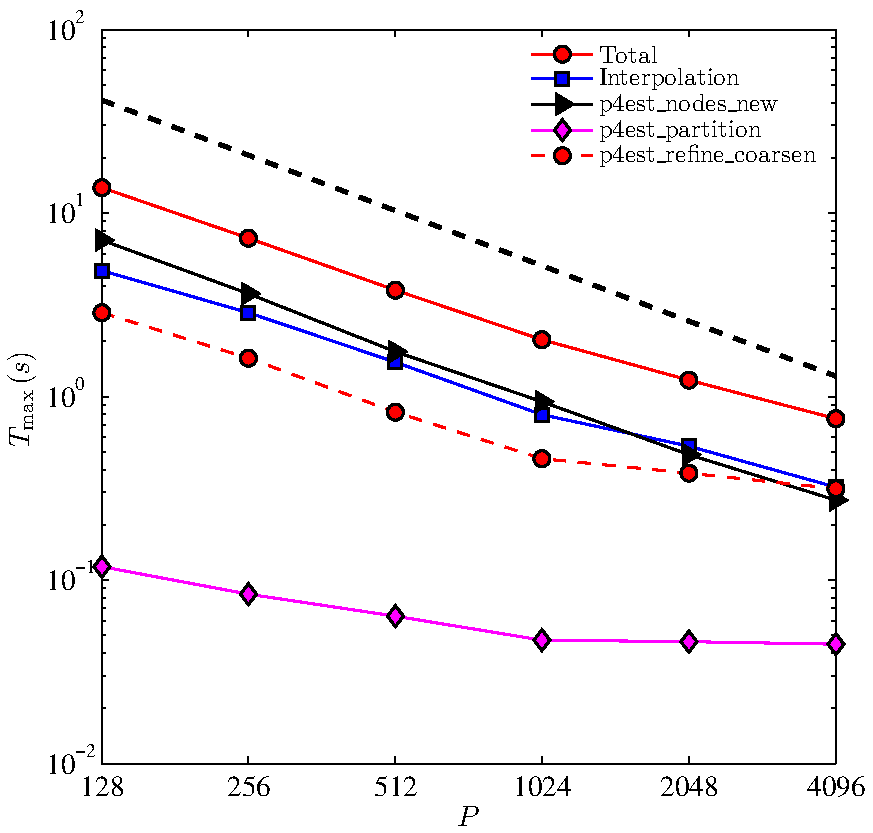
\includegraphics[width = 0.3 \textwidth] {figures/SL_Large_100_SemiLagrangian.pdf}}
		\\
		\subfigure[Interpolation, $\text{CFL} = 1$]{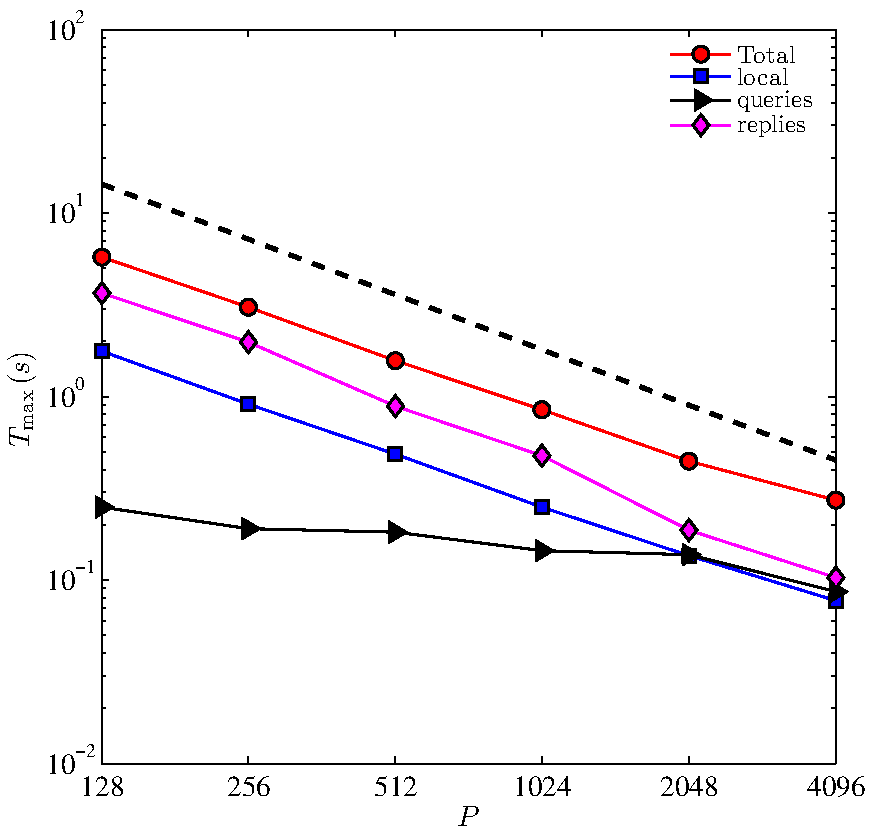
\includegraphics[width = 0.3 \textwidth] {figures/SL_Large_1_Interpolation.pdf}}
		\subfigure[Interpolation, $\text{CFL} = 10$]{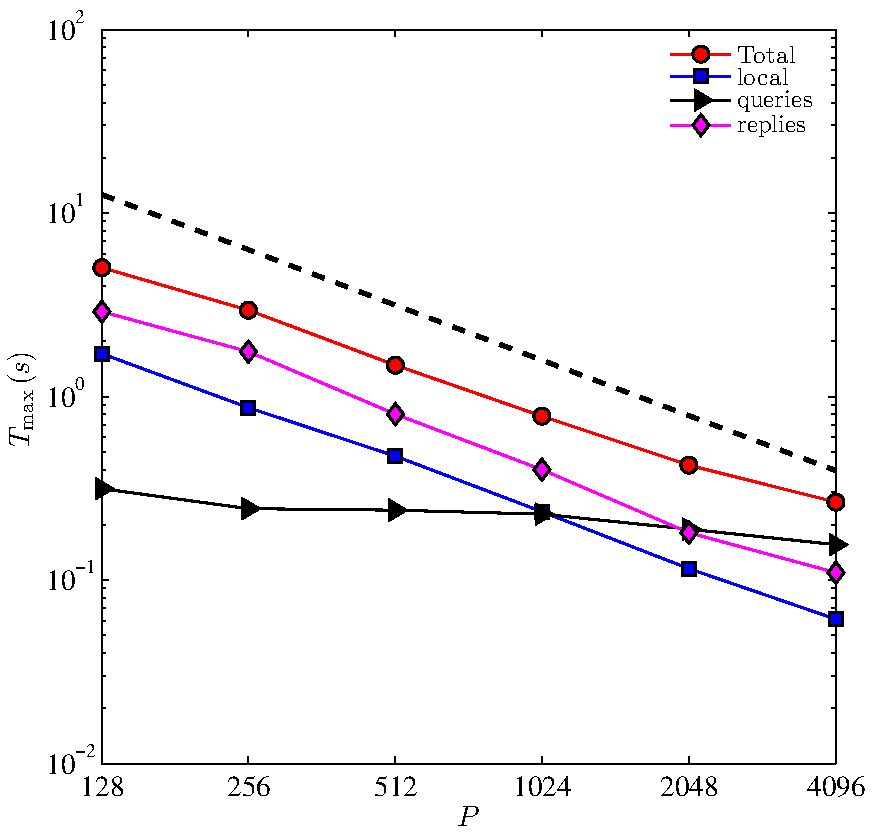
\includegraphics[width = 0.3 \textwidth] {figures/SL_Large_10_Interpolation.pdf}}
		\subfigure[Interpolation, $\text{CFL} = 100$]{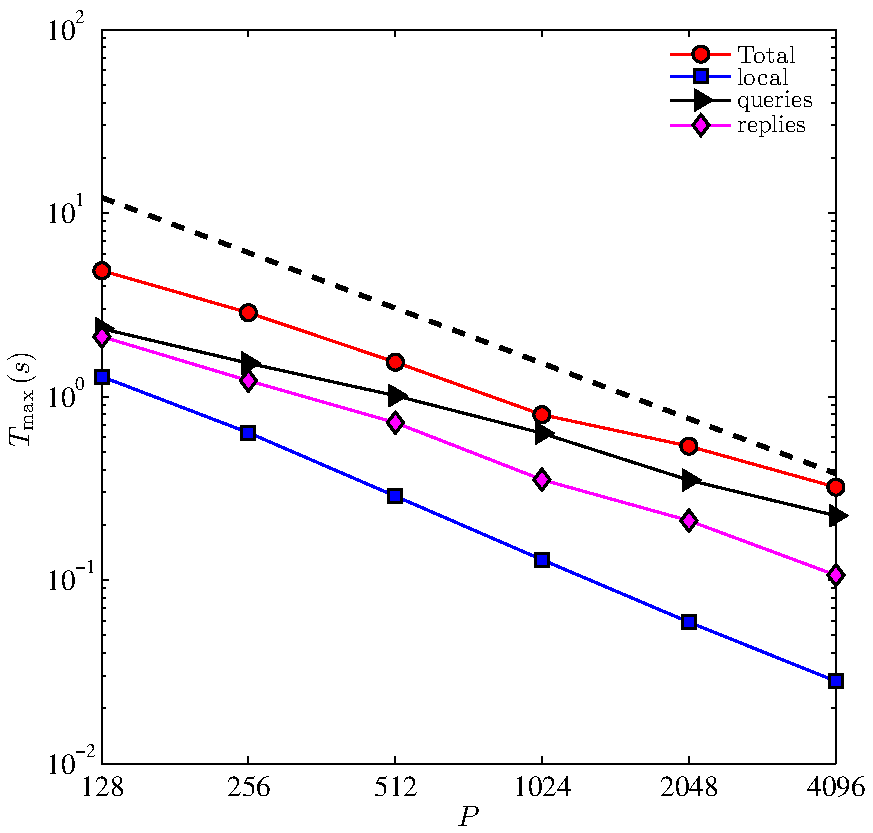
\includegraphics[width = 0.3 \textwidth] {figures/SL_Large_100_Interpolation.pdf}}
	\end{center}
	\caption{Strong scaling of a single iteration of algorithm \ref{alg:semi-lagrangian} for the rotation test on a level-12 Octree with approximately 251M cells and 255M nodes. Top row: scaling of the various components of the algorithm for (a) $\text{CFL} = 1$, (b) $\text{CFL} = 10$, and (c) $\text{CFL} = 100$. Bottom row: breakdown of the various components of the interpolation phase for the same CFL numbers. Note that the maximum time has been scaled by the number of iterations required to build the tree (c.f. table \ref{tab:semilagrangian}).}
	\label{fig:semilagrangian_large}
\end{figure}

To better understand the importance of the CFL number on the scalability, we have recorded a complete history of the communication pattern in the interpolation step. Figure \ref{fig:communication_4096} illustrates the effects of the CFL number on three different metrics, namely the number of interpolation points\footnote{Note that this includes both the local points and the points queried by other processors}, $N_p$, the number of sent and received messages, $N_m = S + R$, and the total communication volume, $V_m$ in mega bytes (MB), for $p=4096$ processors. Furthermore, these values are reported for the first (top row) and last (bottom row) iterations of the Semi-Lagrangian algorithm. There are several points to make. First, increasing the CFL number greatly increases the load imbalance, as shown by the spread of the data in figure \ref{fig:communication_4096_pf}. This is because at higher CFL numbers, and with the velocity field prescribed, it is more likely that some processors will receive a larger portion of the backtracked points. Second, increasing the CFL number increases both the communication volume and its spread across processors (c.f. figure \ref{fig:communication_4096_vf}). Interestingly, however, the number of messages sent and received seems to be unaffected by the CFL number. The bottom row of figure \ref{fig:communication_4096} exhibits a better balance both in the computation and communication volume in the last iteration of the Semi-Lagrangian algorithm. This can be explained by noting that as the algorithm converges to the final grid, partitioning of the grid essentially becomes equivalent to partitioning of the backtracked points \comment{awkward ... maybe: the partitioning of the the grids $G^n$ and $G^{n+1}$ become very similar ?}. Detailed information about the load balancing and the communication patterns is listed in table \ref{tab:communication}.
\begin{figure}[htbp]
	\begin{center}
		\subfigure[]{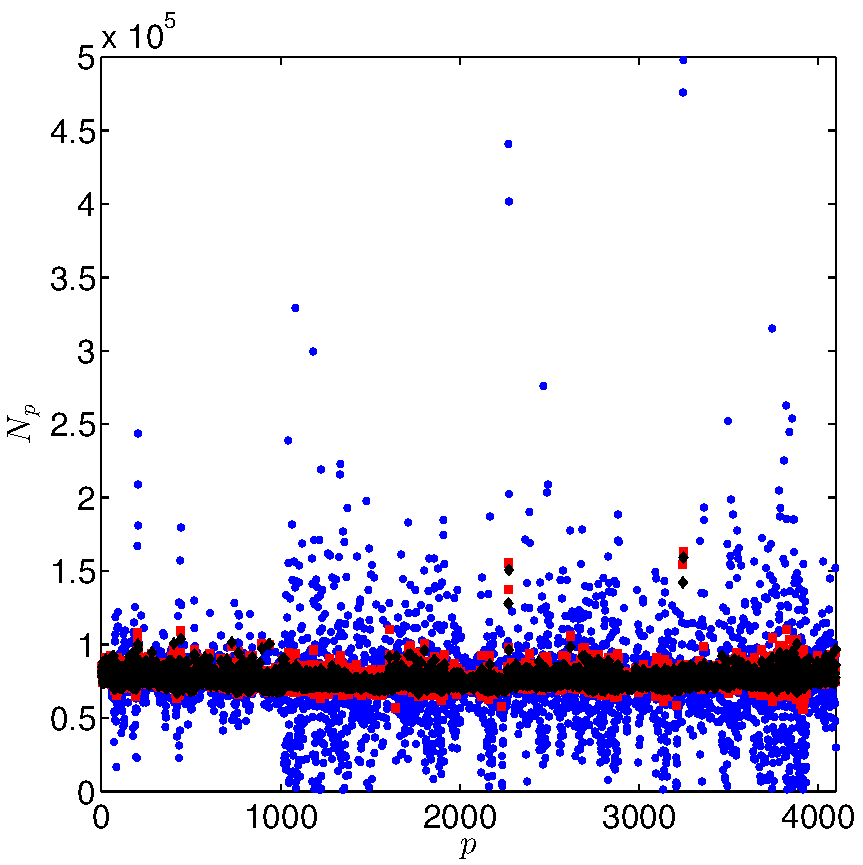
\includegraphics[width = 0.3 \textwidth] {figures/point_first_4096.pdf}  \label{fig:communication_4096_pf}}
		\subfigure[]{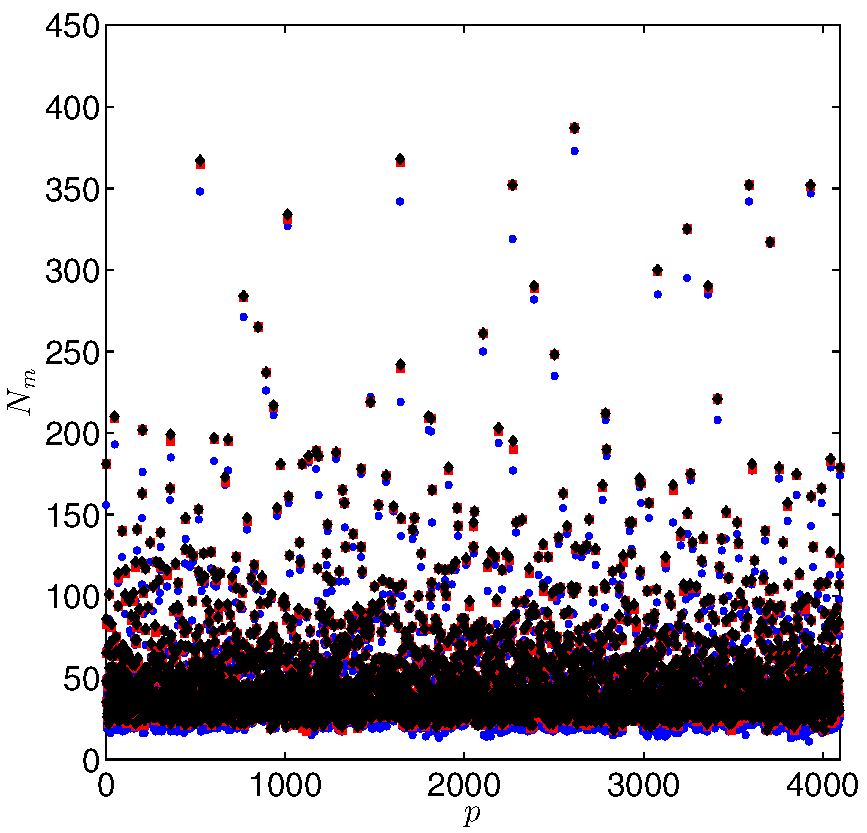
\includegraphics[width = 0.3 \textwidth] {figures/message_first_4096.pdf}\label{fig:communication_4096_mf}}
		\subfigure[]{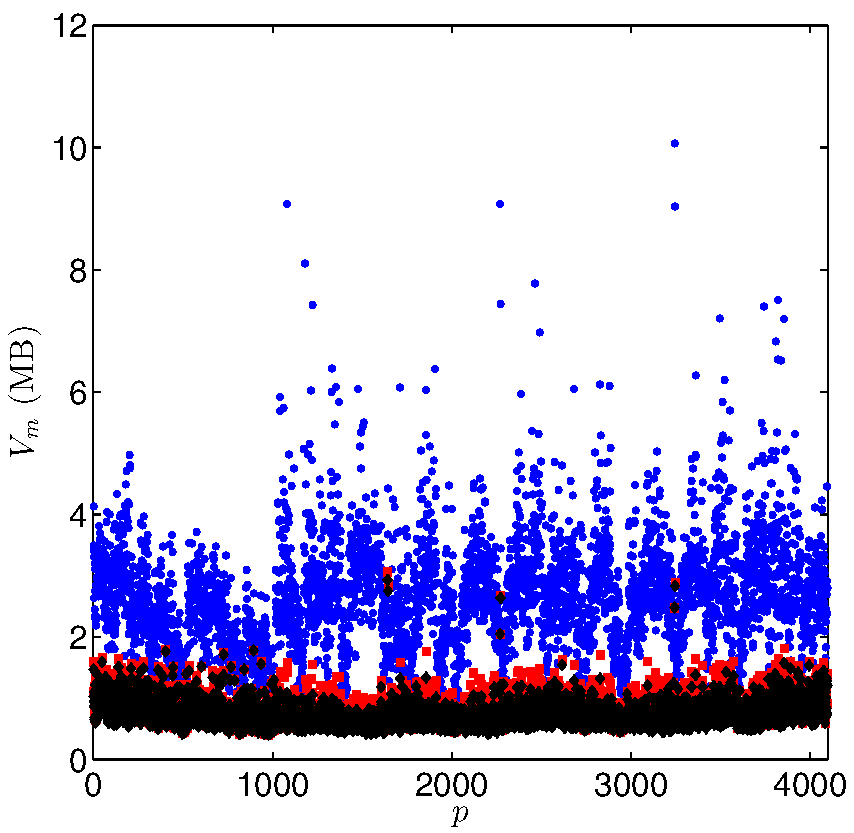
\includegraphics[width = 0.3 \textwidth] {figures/volume_first_4096.pdf} \label{fig:communication_4096_vf}}
		\\
		\subfigure[]{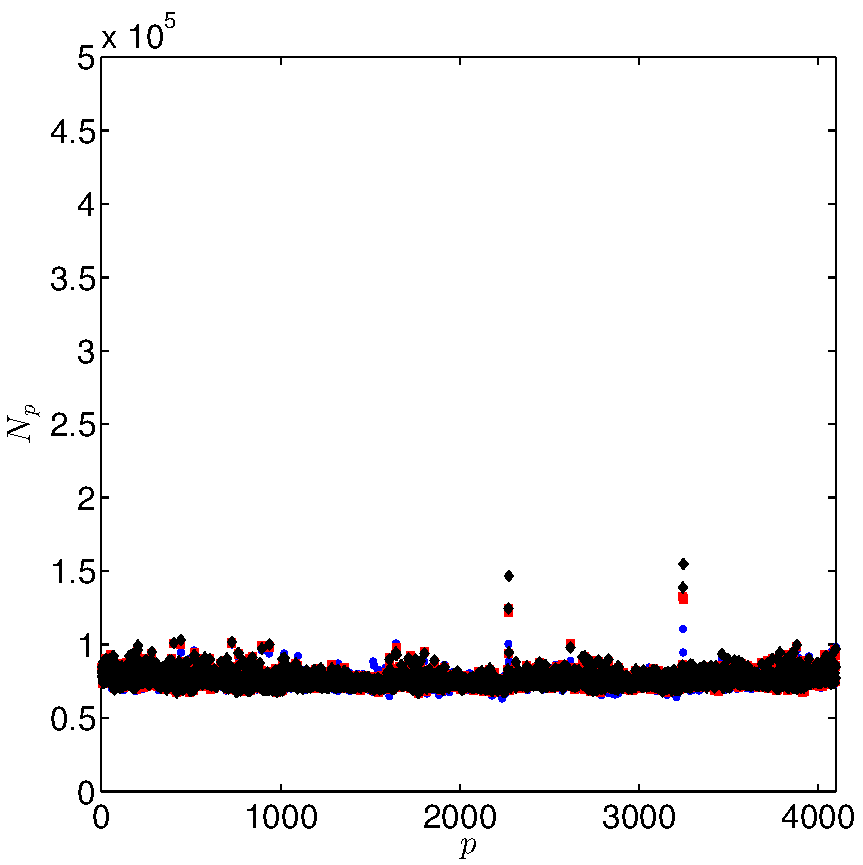
\includegraphics[width = 0.3 \textwidth] {figures/point_last_4096.pdf}   \label{fig:communication_4096_pl}}
		\subfigure[]{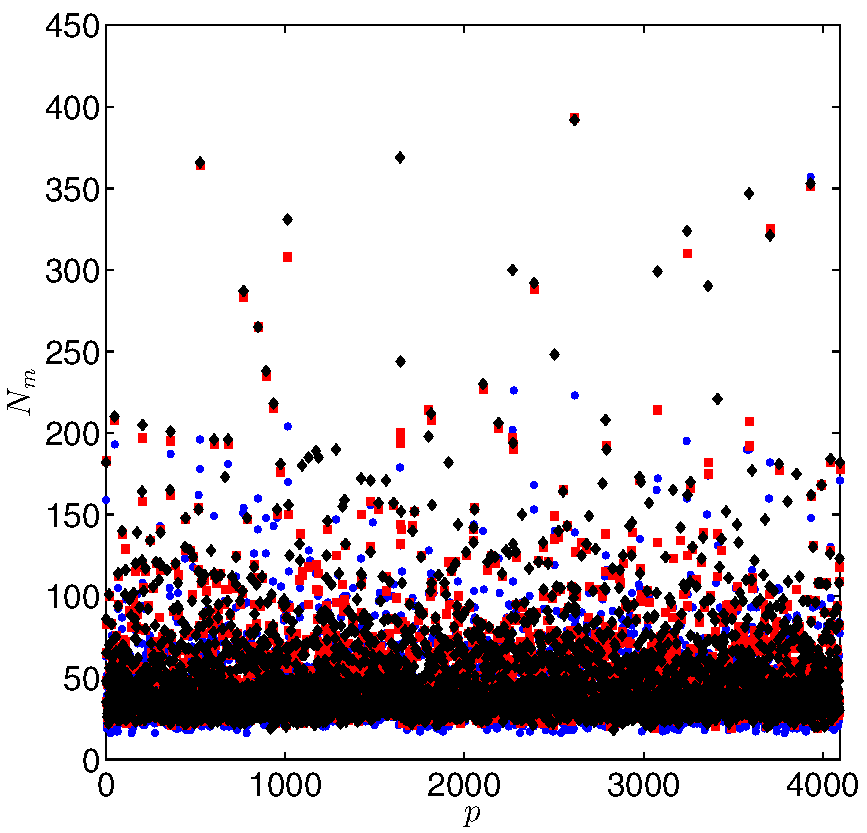
\includegraphics[width = 0.3 \textwidth] {figures/message_last_4096.pdf} \label{fig:communication_4096_ml}}
		\subfigure[]{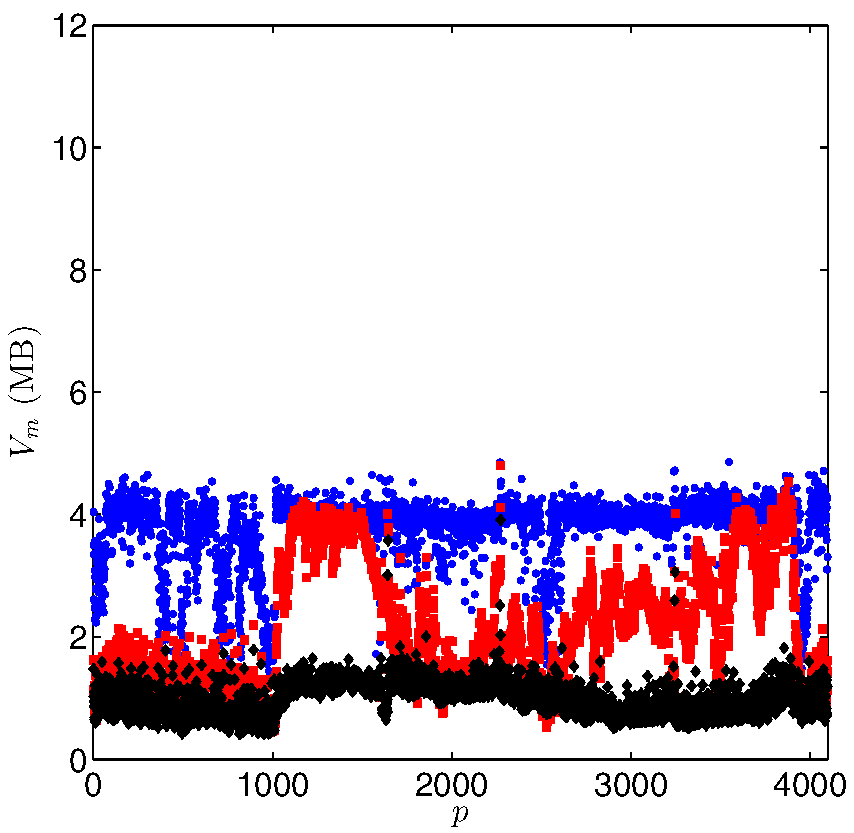
\includegraphics[width = 0.3 \textwidth] {figures/volume_last_4096.pdf}  \label{fig:communication_4096_vl}}		
	\end{center}
	\caption{Performance indicators of the first (top row) and last (bottom row) iterations of the Semi-Lagrangian algorithm for the advection on 4096 processors with $\text{CFL} = 1$ (\drawdiamond{black} \comment{this does not work on my computer, I see a W}), $\text{CFL} = 10$ (\drawsquare{red}), and $\text{CFL} = 100$ (\drawcircle{blue}). Increasing the CFL number greatly causes load imbalance during interpolation (a) and increases the communication volume (c). However, the CFL number does not seem to appreciably affect the number of messages sent by the processors (b). During the last Semi-Lagrangian iteration, the initial grid $G_0$ (c.f. algorithm \ref{alg:semi-lagrangian}) is very close to the final grid. As a result, the load imbalance is considerably improved (d). Curiously, however, the communication pattern does not seem to be change much between first and last iterations (e-f) \comment{e-f ?}.}
	\label{fig:communication_4096}
\end{figure}

\begin{table}[htbp]
	\centering
	\resizebox{\columnwidth}{!}{
	\begin{tabular}{|c|c|cccc|cccc|}
	\hline
	\multirow{2}{*}{CFL} & \multirow{2}{*}{Metric} & \multicolumn{4}{|c|}{First Iteration} & \multicolumn{4}{|c|}{Last Iteration} \\
	\cline{3-10}
											 & 												 & min & max & avg & stddev 					   & min & max & avg & stddev 						\\
	\hline
	\multirow{3}{*}{1}   & $N_p$        & 6.67E+04 & 1.59E+05 & 7.57E+04 & 4.86E+03 & 6.69E+04 & 1.55E+05 & 7.57E+04 & 4.73E+03 \\
										   & $N_m$ 			  & 18 			 & 387 		  & 47.55 	 & 31.72 		& 18 			 & 392 			& 47.55 	 & 31.19 		\\
										   & $V_m$ (MB)   & 4.01E-01 & 2.93E+00 & 7.25E-01 & 1.95E-01 & 4.13E-01 & 3.91E+00 & 9.68E-01 & 2.62E-01 \\
										   & $T_{\max}$ (s) & \multicolumn{4}{|c|}{6.96E-01}						& \multicolumn{4}{|c|}{3.67E-01}						\\
	\hline
	\multirow{3}{*}{10}  & $N_p$        & 5.56E+04 & 1.63E+05 & 7.57E+04 & 6.07E+03 & 6.65E+04 & 1.33E+05 & 7.57E+04 & 4.50E+03 \\
										   & $N_m$ 			  & 17 			 & 387 		  & 46.73 	 & 31.78 		& 19 			 & 393 			& 46.68 	 & 27.93 		\\
										   & $V_m$ (MB)   & 4.01E-01 & 3.06E+00 & 8.40E-01 & 2.21E-01 & 4.40E-01 & 4.80E+00 & 2.14E+00 & 9.88E-01 \\
											 & $T_{\max}$ (s) & \multicolumn{4}{|c|}{7.55E-01}						& \multicolumn{4}{|c|}{3.30E-01}						\\
	\hline
	\multirow{3}{*}{100} & $N_p$        & 8.28E+02 & 4.98E+05 & 7.57E+04 & 3.14E+04 & 6.30E+04 & 1.10E+05 & 7.57E+04 & 4.20E+03 \\
										   & $N_m$ 			  & 11 			 & 373 		  & 41.18 	 & 30.85 		& 16 			 & 357 			& 41.77 	 & 22.66 		\\
										   & $V_m$ (MB)   & 5.28E-01 & 1.01E+01 & 2.65E+00 & 9.24E-01 & 9.76E-01 & 4.86E+00 & 3.78E+00 & 5.69E-01 \\
											 & $T_{\max}$ (s) & \multicolumn{4}{|c|}{9.25E-01}						& \multicolumn{4}{|c|}{3.55E-01}						\\
	\hline
	\end{tabular}
	}
	\caption{Detailed load balancing and communication information for the advection test problem for $\text{CFL} = 1$, $\text{CFL} = 10$, and $\text{CFL} = 100$. Note how increasing the CFL number causes load imbalance and increases the communication volume while it does not affect the number of messages sent and received during an iteration of the Semi-Lagrangian step.}
	\label{tab:communication}
\end{table}

\subsection{Reinitialization} \label{section::scaling_reinitialization}

Finally we present the scaling results of our parallel reinitialization algorithm where we extensively make use of algorithm \ref{alg:overlap} for overlapping computation with communication when computing spatial derivatives. Our test consists in computing the signed distance to a collection of 100 spheres, whose radii and centers have been chosen randomly. The test is performed on a small, level-8 Octree with nearly 21M and a larger, level-10 Octree with nearly 337M grid points. In both cases the forest is built on a $3\times3\times3$ macro-mesh. Figure \ref{fig:reinit} illustrates that our reinitialization algorithm, and in particular the overlapping strategy presented in algorithm \ref{alg:overlap}, scales very well. In general we expect similar scaling results for any local, finite-difference based calculations on Octrees that can efficiently utilize algorithm \ref{alg:overlap}. 
\begin{figure}
\centering
\subfigure[]{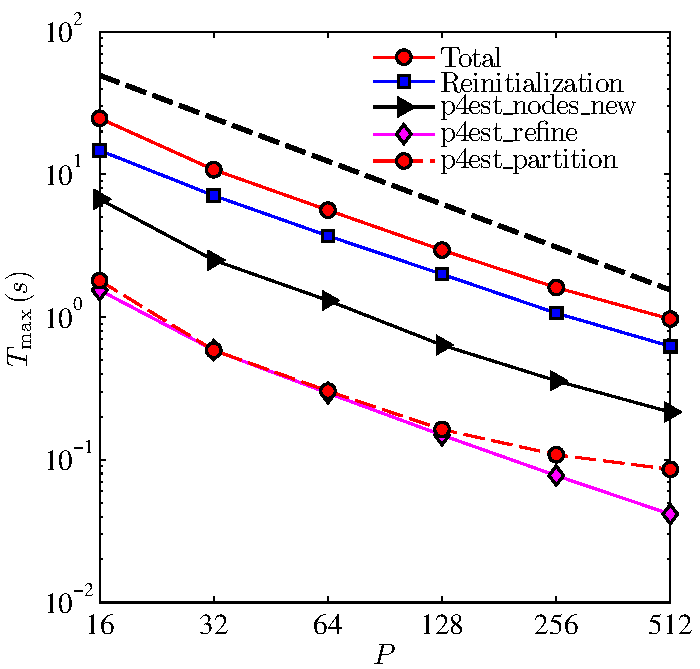
\includegraphics[width=0.45\textwidth]{figures/Reinit_Small.pdf}}
\subfigure[]{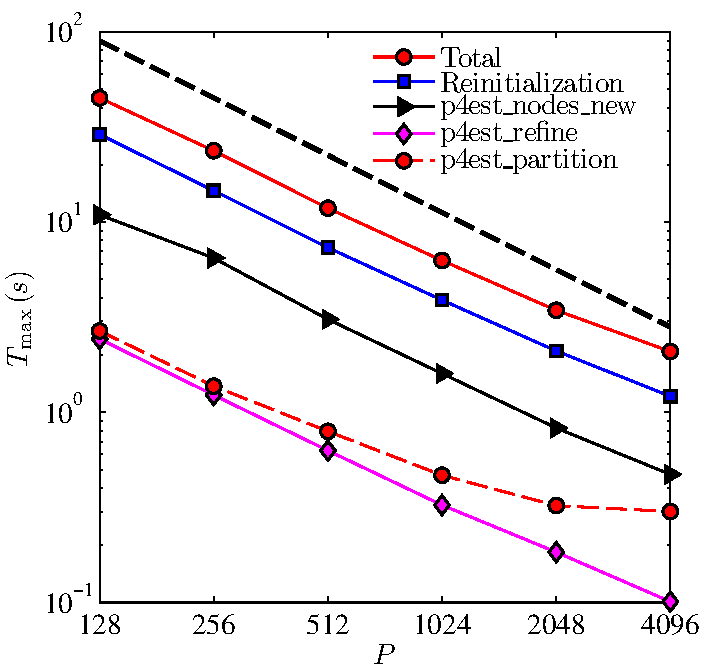
\includegraphics[width=0.45\textwidth]{figures/Reinit_Large.pdf}}
\caption{Scalability of the reinitialization test for a small (left) and large (right) Octree with roughly 21M and 337M grid points, respectively. Excellent results are obtained in both cases, illustrating the scalability of the overlapping strategy (c.f. algorithm \ref{alg:overlap}).}
\label{fig:reinit}
\end{figure}
